\subsection{Scenario classes}
\label{sec:scenario classes}
% Introduce term scenario class (i.e. qualitative description of scenario)
In this section, the notion of scenario class is introduced. As proposed above, a scenario in the context of the performance assessment of an AV needs to be quantitative. There exists, however, a qualitative description of each scenario. The qualitative description can be regarded as an abstraction of the quantitative scenario. As a result, for a qualitative description there may be an infinite amount of scenarios. A scenario class is a qualitative description of a scenario. 

% Name different names of traffic scenarios in literature
In literature, many different types of scenarios are considered, such as a cut-in \cite{xu2002effects, gietelink2006development,roesener2017comprehensive}, braking of a predecessor \cite{xu2002effects,deGelder2017assessment,hulshof2013autonomous}, a near miss \cite{gietelink2006development}, a collision or a safety-critical scenario \cite{gietelink2006development,ebner2011identifying}, an urban scenario \cite{zofka2015datadrivetrafficscenarios}, a free-driving or vehicle-following scenario \cite{roesener2017comprehensive}, a lane change \cite{roesener2017comprehensive}, an overtaking \cite{karaduman2013interactivebehavior}, a platoon merge \cite{englund2016grand}, an intersection passing \cite{englund2016grand}, a highway lane reduction \cite{ploeg2017GCDC}, or urban intersection crossing \cite{ploeg2017GCDC}. In order to get a complete picture of all scenarios that are encountered in traffic, this list of scenarios should be expanded. However, when doing this, the following problems occur:

% Problems: not mutually exclusive, not complete, depends
\begin{enumerate}
	\item The scenario classes are not mutually exclusive, so it is unclear how a scenario should be classified. For example, a scenario in which a predecessor brakes can be both a braking scenario and an urban scenario. \label{item:mutual exclusiveness}
	\item It might be difficult to determine whether the list of scenarios is complete. A more structured approach is necessary for this. \label{item:completeness}
	\item There is a balance between general scenario classes - and thus a high variety - and specific scenario classes - and thus not much variety. For example, for some systems one is interested in cut-in scenarios on highways, while for another system one might be interested in cut-in scenarios on all road types. \label{item:generality}
\end{enumerate}

% Solution
The proposed solution is to provide tree structure of tags that describe the scenario. A tag could be something that describes the weather, the type of road or a specific activity of a target vehicle, etc. The tags are structured according to different trees, see Figure~\ref{fig:tag trees} for four examples. Tags that are in the same layer or tags that are in different branches are mutually exclusive. For example, regarding the weather (Figure~\ref{fig:tag trees}a), it is not possible to have a scenario in which there is rain and snow at the same time. The different layers of the trees can be regarded as different abstraction levels \cite{Bonnin2014}. 

The trees provide the possibility to define specific tags, while these specific tags belong to a more generic tag. For example, when examining the following behavior of an automated vehicle, one might want to test for all vehicle-following scenarios (see Figure~\ref{fig:tag trees}b), while in another case one might want to only test for the vehicle-following scenarios with braking involved when testing the braking capability of the automated system in a vehicle-following scenario.

Note that the tags assigned to the scenario may depend on the ego vehicle. For example, the `target in front' refers to the vehicle in front of the ego vehicle.

\begin{figure}
	\begin{center}
		\tikzstyle{tag}=[text height=.8em, text depth=.1em, fill=gray!20, rounded corners=0.2em]
		\tikzstyle{helper}=[coordinate, node distance=1.4em]
		\subfloat[Tags for weather condition, see \cite{mahmassani2012use}.]{
			\definecolor{TNOlightgray}{RGB}{222,222,231}%
\tikzstyle{tag}=[font=\sffamily, text height=.8em, text depth=.1em, fill=TNOlightgray, rounded corners=0.2em]%
\tikzstyle{helper}=[coordinate, node distance=1.4em]%
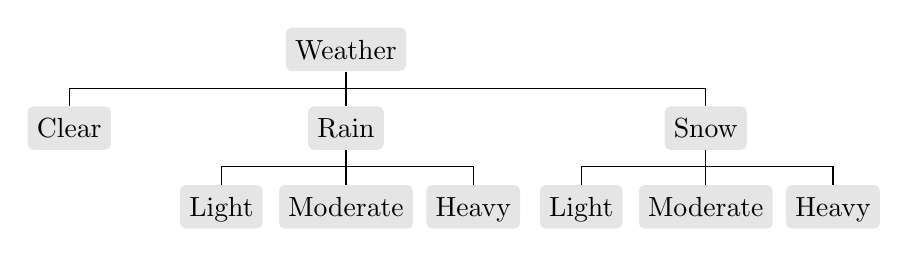
\begin{tikzpicture}
	% Place the nodes
	\node[tag](weather){Weather};
	\node[tag, below of=weather](rain){Rain};
	\node[tag, left of=rain, node distance=10em](clear){Clear};
	\node[tag, right of=rain, node distance=13em](snow){Snow};
	\node[tag, below of=rain](mod rain){Moderate};
	\node[tag, left of=mod rain, node distance=4.5em](light rain){Light};
	\node[tag, right of=mod rain, node distance=4.6em](heavy rain){Heavy};
	\node[tag, below of=snow](mod snow){Moderate};
	\node[tag, left of=mod snow, node distance=4.5em](light snow){Light};
	\node[tag, right of=mod snow, node distance=4.6em](heavy snow){Heavy};
	
	% Place the lines
	\node[helper, below of=weather](weather helper){};
	\node[helper, below of=rain](rain helper){};
	\node[helper, below of=snow](snow helper){};
	\draw (weather) -- (rain);
	\draw (weather) -- (weather helper) -| (clear);
	\draw (weather) -- (weather helper) -| (snow);
	\draw (rain) -- (mod rain);
	\draw (rain) -- (rain helper) -| (light rain);
	\draw (rain) -- (rain helper) -| (heavy rain);
	\draw (snow) -- (mod snow);
	\draw (snow) -- (snow helper) -| (light snow);
	\draw (snow) -- (snow helper) -| (heavy snow);
\end{tikzpicture}%

		} \\
		\subfloat[Tags for target description.]{
			\definecolor{TNOlightgray}{RGB}{222,222,231}%
\tikzstyle{tag}=[font=\sffamily, text height=.8em, text depth=.1em, fill=TNOlightgray, rounded corners=0.2em]%
\tikzstyle{diffheighttag}=[node distance=2.5em]%
\tikzstyle{helper}=[coordinate, node distance=1.5em]%
\tikzstyle{helper2}=[coordinate, node distance=4.0em]%
\begin{tikzpicture}
	% Place the nodes
	\node[tag](target){\footnotesize Target in front};
	\node[coordinate, below of=target](below target){};
	\node[coordinate, left of=below target, node distance=3.4em](following){};
	\node[tag, diffheighttag, below of=following](following2){\footnotesize Vehicle following};
	\node[tag, left of=following, node distance=3.5em](free){\footnotesize No target};
	\node[tag, right of=below target, node distance=4.4em](appearing){\footnotesize Target appearing};
	\node[coordinate, right of=appearing, node distance=4.5em](disappearing){};
	\node[tag, diffheighttag, below of=disappearing](disappearing2){\footnotesize Target disappearing};
	\node[coordinate, below of=following2, node distance=2.8em](braking){};
	\node[tag, diffheighttag, below of=braking](braking2){\footnotesize Braking};
	\node[tag, left of=braking2, node distance=3.7em](cruising){\footnotesize Cruising};
	\node[tag, right of=braking2, node distance=4.4em](accelerating){\footnotesize Accelerating};
	\node[coordinate, below of=appearing](below appearing){};
	\node[coordinate, diffheighttag, below of=below appearing](below appearing2){};
	\node[tag, left of=below appearing2, node distance=2.6em](cutin){\footnotesize Cut-in};
	\node[tag, right of=below appearing2, node distance=1.5em](gapclosing){\footnotesize Gap-closing};
	\node[coordinate, below of=disappearing2](below disappearing){};
	\node[coordinate, diffheighttag, below of=below disappearing](below disappearing2){};
	\node[tag, left of=below disappearing2, node distance=2.3em](cutout){\footnotesize Cut-out};
	\node[tag, right of=below disappearing2, node distance=2.3em](gapmaking){\footnotesize Gap-making};
	
	% Place the lines
	\node[helper, below of=target](target helper){};
	\node[helper2, below of=following2](following helper){};
	\node[helper2, below of=appearing](appearing helper){};
	\node[helper2, below of=disappearing2](disappearing helper){};
	\draw (target) -- (target helper) -| (free);
	\draw (target) -- (target helper) -| (following2);
	\draw (target) -- (target helper) -| (appearing);
	\draw (target) -- (target helper) -| (disappearing2);
	\draw (following2) -- (following helper) -| (cruising);
	\draw (following2) -- (braking2);
	\draw (following2) -- (following helper) -| (accelerating);
	\draw (appearing) -- (appearing helper) -| (cutin);
	\draw (appearing) -- (appearing helper) -| (gapclosing);
	\draw (disappearing2) -- (disappearing helper) -| (cutout);
	\draw (disappearing2) -- (disappearing helper) -| (gapmaking);
\end{tikzpicture}%

		}\\
		\subfloat[Tags for type of road, inspired from \cite{Bonnin2014}.]{
			\definecolor{TNOlightgray}{RGB}{222,222,231}%
\tikzstyle{tag}=[font=\sffamily, text height=.8em, text depth=.1em, fill=TNOlightgray, rounded corners=0.2em]%
\tikzstyle{helper}=[coordinate, node distance=1.4em]%
\tikzstyle{emph}=[fill=TNOred]
\begin{tikzpicture}
	% Place the nodes
	\node[tag, emph](road){Type of road};
	\node[coordinate, below of=road](below road){};
	\node[tag, left of=below road, node distance=10em, emph](highway){Highway};
	\node[tag, right of=below road, node distance=9.5em](inner city){Inner city};
	\node[tag, right of=inner city, node distance=10.5 em](remaining a){...};
	\node[coordinate, below of=highway](below highway){};
	\node[tag, left of=below highway, node distance=2em](exit){Exit};
	\node[tag, left of=exit, node distance=4em](entrance){Entrance};
	\node[tag, right of=below highway, node distance=2em, emph](merging highway){Merging};
	\node[tag, right of=merging highway, node distance=3.4em](remaining b){...};
	\node[tag, below of=inner city](intersection){Intersection};
	\node[tag, left of=intersection, node distance=8em](pedestrian crossing){Pedestrian crossing};
	\node[tag, right of=intersection, node distance=5.6em](merging inner city){Merging};
	\node[tag, right of=merging inner city, node distance=3.5em](remaining c){...};
	
	% Place the lines
	\node[helper, below of=road](road helper){};
	\node[helper, below of=highway](highway helper){};
	\node[helper, below of=inner city](inner city helper){};
	\draw (road) -- (road helper) -| (highway);
	\draw (road) -- (road helper) -| (inner city);
	\draw (road) -- (road helper) -| (remaining a);
	\draw (highway) -- (highway helper) -| (entrance);
	\draw (highway) -- (highway helper) -| (exit);
	\draw (highway) -- (highway helper) -| (merging highway);
	\draw (highway) -- (highway helper) -| (remaining b);
	\draw (inner city) -- (inner city helper) -| (pedestrian crossing);
	\draw (inner city) -- (intersection);
	\draw (inner city) -- (inner city helper) -| (merging inner city);
	\draw (inner city) -- (inner city helper) -| (remaining c);
\end{tikzpicture}%

		} \\
		\subfloat[Tags for the criticality, see \cite{ebner2011identifying}.]{
			\input{figures/tree_criticality.tikz}
		}
		\caption{Examples of tree structures with \emph{tags} for a scenario.}
		\label{fig:tag trees}
	\end{center}
\end{figure}
